\documentclass{standalone}
\usepackage{tikz}

\begin{document}
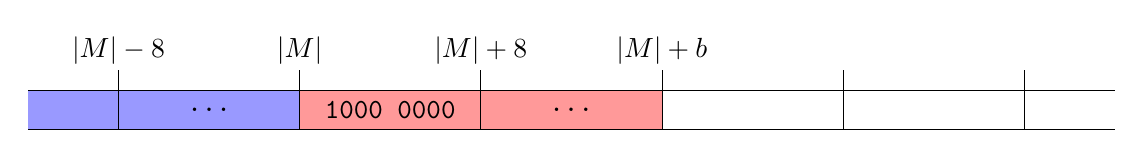
\begin{tikzpicture}[xscale=2.3,yscale=0.5]
\fill[blue!40!white]  (-0.5,0.0) rectangle (1.0,1.0);
\fill[red!40!white]   ( 1.0,0.0) rectangle (3.0,1.0);

\draw[step=1cm,black,very thin] (-0.5,0.0) grid (5.5,1.5);
\node at (0.5,0.5) {\tt{...}};
\node at (1.5,0.5) {\tt{1000 0000}};
\node at (2.5,0.5) {\tt{...}};

\node at (0.0,2.0) {$|M|-8$};
\node at (1.0,2.0) {$|M|$};
\node at (2.0,2.0) {$|M|+8$};
\node at (3.0,2.0) {$|M|+b$};
\end{tikzpicture}
\end{document}